% LTeX: language=de-DE
\section{Tree-walking Interpreter}

\begin{frame}{Tree-walking Interpreter}
	\pdfpcnote{
		@Silas \\
		\\
		- Ein tree-walking Interpreter funktioniert so, dass er den analysierten Syntaxbaum _traversiert_ \\
		- und ohne weitere Zwischenschritte die Anweisungen _interpretiert_ \\
	}

	\begin{itemize}
		\item \emph{Traversiert} den Syntaxbaum
		\item \emph{Interpretiert} das Programm direkt
	\end{itemize}
\end{frame}

\begin{frame}{Felder des Interpreters}
	\pdfpcnote{
		@Silas \\
		\\
		- Typdefinition des Interpreters \\
		- Aufbau sehr simpel: benoetigt nur zwei Felder \\
		- scopes: Zuweisung von Variablennamen zu Laufzeitwerten \\
		- functions: Zuweisung von Funktionsnamen zu dem Knoten des Syntaxbaums \\
	}

	\begin{flushright}
		\begin{minipage}{.85\textwidth}
			\Lirsting[float=H, ranges={10-16}, fancyvrb={frame=none, fontsize=\small}]{deps/rush/crates/rush-interpreter-tree/src/interpreter.rs}
		\end{minipage}
	\end{flushright}

	\begin{description}
		\item[scopes] Stack von Scopes; jeder Scope weist einem Variablennamen einen Laufzeitwert zu
		\item[functions] Zuweisung von Funktionsnamen zu dem entsprechenden Knoten im Syntaxbaum
	\end{description}
\end{frame}

\begin{frame}{Laufzeitwerte}
	\pdfpcnote{
		@Silas \\
		\\
		- Laufzeitwerte verschiedener Datentypen werden unter einem allgemeinen Typ zusammengefasst \\
	}

	\centering
	\begin{minipage}{0.37\textwidth}
		\Lirsting[float=H, ranges={6-13}, fancyvrb={frame=none}]{deps/rush/crates/rush-interpreter-tree/src/value.rs}
	\end{minipage}
\end{frame}

\begin{frame}{Traversierung}
	\pdfpcnote{
		@Silas \\
		\\
		- sichtbar: Syntaxbaum zu dem Ausdruck `1 + 2 * 3` \\
		- interessant: Reihenfolge der Traversierung \\
		- post-order \\
		- weil: fuer die Addition muss erst das Produkt von `2 * 3` berechnet werden \\
	}

	\begin{figure}[H]
		\centering
		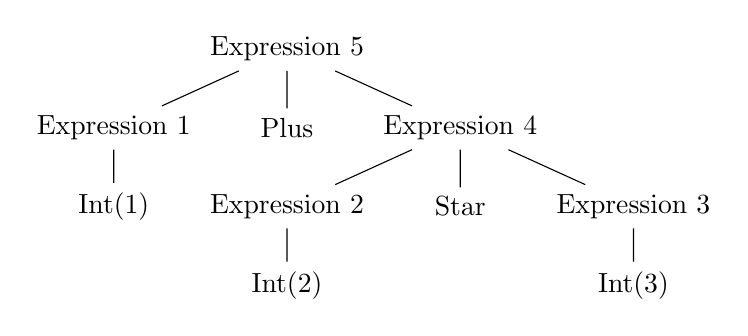
\begin{tikzpicture}[level distance=1cm, sibling distance=2.2cm, transform shape]
			\node {Expression \encircle{5}}
			child {node {Expression \encircle{1}}
					child {node {\Verb{Int(1)}}}}
			child {node {\Verb{Plus}}}
			child {node {Expression \encircle{4}}
					child {node {Expression \encircle{2}}
							child {node {\Verb{Int(2)}}}}
					child {node {\Verb{Star}}}
					child {node {Expression \encircle{3}}
							child {node {\Verb{Int(3)}}}}};
		\end{tikzpicture}
		\caption{Syntaxbaum zu \enquote{\LirstInline{rush}{1 + 2 * 3}}}
	\end{figure}
\end{frame}

\begin{frame}{Effizienz}
	\pdfpcnote{
		@Silas \\
		\\
		- Beispiel: das bereits gezeigte rekursive Fibonacci Programm \\
		- Grafik rechts: Funktionsaufrufe im Interpreter zu einem Zeitpunkt waehrend der Ausfuehrung \\
		- tiefer ist aktueller / neuer \\
		- Ineffizienz durch staendiges verfolgen von Pointern zu anderen Knoten im Baum \\
		- besonders bei rekursiven Programmen, wiederholte Traversierung derselben Knoten \\
		- in diesem Beispiel: der obere Block an aufrufen ist nach jedem Aufruf (bei jedem "...") vorhanden \\
	}

	\begin{minipage}{0.5\textwidth}
		\Lirsting[float=H, fancyvrb={frame=none, fontsize=\small}]{deps/paper/listings/fib.rush}
	\end{minipage}
	\hfill
	\begin{minipage}{0.45\textwidth}
		\begin{tikzpicture}
			\scriptsize
			\matrix[
			matrix of nodes,
			nodes={minimum height=3ex, draw, text width=4cm},
			row sep=-\pgflinewidth
			](stack){
			\dots \\
			\LirstInline{rs}{call_func("fib", vec![10])} \\
			\LirstInline{rs}{visit_block(/* ... */)} \\
			\LirstInline{rs}{visit_expression(/* ... */)} \\
			\LirstInline{rs}{visit_if_expr(/* ... */)} \\
			\LirstInline{rs}{visit_block(/* ... */)} \\
			\LirstInline{rs}{visit_expression(/* ... */)} \\
			\LirstInline{rs}{visit_inifix_expr(/* ... */)} \\
			\LirstInline{rs}{visit_expression(/* ... */)} \\
			\LirstInline{rs}{visit_call_expr(/* ... */)} \\
			\LirstInline{rs}{call_func("fib", vec![8])} \\
			\dots \\
			\LirstInline{rs}{call_func("fib", vec![6])} \\
			\dots \\
			\LirstInline{rs}{call_func("fib", vec![4])} \\
			\dots \\
			\LirstInline{rs}{call_func("fib", vec![2])} \\
			\dots \\
			\LirstInline{rs}{call_func("fib", vec![0])} \\
			};
			\draw[arrow] ([xshift=1em]stack.north east) -- ([xshift=1em]stack.south east);
		\end{tikzpicture}
	\end{minipage}
\end{frame}
